
\subsection{Esempio Massa-Molla-Smorzatore con due masse}
Si vuole analizzare il modello ISU del seguente sistema composto da due masse
disposte nel seguente modo:
\begin{figure}[h]
 \centering
 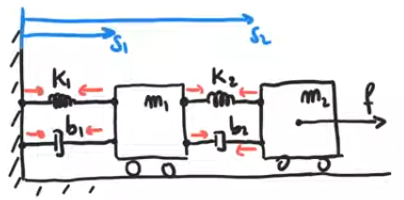
\includegraphics[width=\picwid]{massa_molla_smorzatore_esempio_2.png}
 \label{fig:massa_molla_smorzatore_esempio_2}
\end{figure}

Si individua il sistema di riferimento e si indica con $s_1$ la posizione della
prima massa ed $s_2$ la seconda.
Esiste un'unica direzione di movimento e sono presenti due masse, dunque si
scriveranno due equazioni.
$$\left\{\begin{aligned}
m_1\ddot{s}_1 &= k_2(s_2-s_1) + b_2(\dot{s}_2-\dot{s}_1) -k_1s_1 - b_1\dot{s}_1
\\
m_2\ddot{s}_2 &= f - k_2(s_2-s_1) - b_2(\dot{s}_2-\dot{s}_1)
\end{aligned}\right.$$

Si analizzano le variabili del sistema
$$\begin{matrix}
f & s_1& \dot{s}_1 & s_2 &\dot{s}_2 \\
(0) & (2) & & (2) \\
u & x_1 & x_2 & x_3 & x_4
\end{matrix}$$

L'ordine del sistema è dunque quattro $(n=4)$, dato che ogni variabile non di
ingresso viene differenziata due volte.

Si riscrivono le equazioni in forma ISU
$$\left\{\begin{aligned}
\dot{x}_1 &= \dot{s}_1 = x_2 \\
\dot{x}_2 &= \ddot{s}_1 = \frac{k_2}{m_1}(x_3-x_1) + \frac{b_2}{m_1} (x_4-x_2)
- \frac{k_1}{m_1}x_1 - \frac{b_1}{m_1}x_2\\
\dot{x}_3 &=\dot{s}_2 = x_4 \\
\dot{x}_4 &= \ddot{s}_2 = \frac{1}{m_2}u -\frac{k_2}{m_2}(x_3-x_1) -
\frac{b_2}{m_2}(x_4 - x_2)\\
\ &\text{Uscite assegnate}\\
y_1 &= s_1 = x_1 \\
y_2 &= s_2 = x_3
\end{aligned}\right.$$

\newpage
Il sistema è lineare tempo invariante strettamente causale, si può porre il
sistema in forma matriciale compatta
$$x =
\begin{pmatrix}
 x_1 \\ x_2 \\ x_3 \\ x_4
\end{pmatrix} \quad
y= \begin{pmatrix}
    y_1 \\ y_2
   \end{pmatrix}
$$
$$\text{ISU} = \left\{\begin{aligned}
\dot{x} &= \begin{pmatrix}
0 & 1 & 0 & 0 \\
\\
-\frac{k_1+k_2}{m_1} & -\frac{b_1+b_2}{m_1} &
\frac{k_2}{m_1} & \frac{b_2}{m_1}\\
\\
0 & 0 & 0 & 1\\ \\
\frac{k_2}{m_2} & \frac{b_2}{m_2} & -\frac{k_2}{m_2} & -\frac{b_2}{m_2}
          \end{pmatrix}x +
          \begin{pmatrix}
        0 \\ 0 \\ 0 \\ \frac{1}{m}
          \end{pmatrix}u\\
y &=      \begin{pmatrix}
           1 & 0 & 0 & 0 \\
           0 & 0 & 1 & 0
          \end{pmatrix}x
\end{aligned}\right.$$

\subsection{Moto rotazionale}
Si considera un primo asse di movimento caratterizzato da una certa inerzia
$J_1$, connesso ad un secondo asse di momento $J_2$ mediante un elemento
elastico di costante $k$.

Si suppone che il primo asse subisca un effetto di attrito viscoso mediante un
coefficiente $b_1$ mentre il secondo subisce un attrito con coefficiente $b_2$.

Si suppone di applicare una coppia \textit{motrice} $\tau_m$ al primo asse ed
una coppia resistente $\tau_r$ in verso opposto al secondo asse.
%% Inserisci figura
\begin{figure}[h]
 \centering
 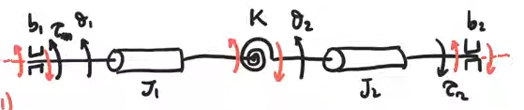
\includegraphics[width=0.6\linewidth]{rotativo_2_assi.png}
 % rotativo_2_assi.png: 524x110 px, 96dpi, 13.86x2.91 cm, bb=0 0 393 82
 \label{Fig.:rotativo_due_assi}
\end{figure}

Questo schema può rappresentare un esempio di accoppiamento non perfettamente
rigido tra l'asse di un motore ed un montacarichi (o un ascensore).
Si suppone il verso positivo degli spostamenti quello concorde con la coppia
$\tau_1$.

Si analizzano le equazioni, ne serviranno due, data la presenza di due inerzie.

$$\left\{\begin{aligned}
J_1 \ddot{\theta}_1 &= \tau_m + k(\theta_2 -\theta_1) - b_1\dot{\theta}_1 \\
J_2 \ddot{\theta}_2 &= -k(\theta_2-\theta_1) +b_2(-\dot{\theta}_2) - \tau_r
\end{aligned}\right.$$

Si sostituiscono le variabili
$$\begin{matrix}
\tau_m & \tau_3 & \theta_1 & \dot{\theta}_1 & \theta_2 & \dot{\theta}_2\\
(0) & (0) &       (2)  &      &  (2)  \\
  u_1  &  u_2  & x_1 & x_2 & x_3 & x_4
\end{matrix}$$

Si scrive il sistema ISU di ordine quattro
$$\left\{
\begin{aligned}
 \dot{x}_1 & = \dot{\theta}_1 = x_2 \\
 \dot{x}_2 &= \ddot{\theta}_1 = \frac{k}{J_1} (x_3 - x_1) - \frac{b_1}{J_1}
x_2\\
\dot{x}_3 &= \dot{\theta}_2 = x_4 \\
\dot{x}_4 &= \dot{\theta}_2 = -\frac{k}{J_2}(x_3-x_1) - \frac{b_2}{J_2}x_4 -
\frac{1}{J_2}u_2\\
&\text{Uscite}\\
y_1 &= \dot\theta_1 = x_2 \\
y_2 &= \dot\theta_2 = x_4
\end{aligned}
\right.$$

Il sistema è lineare tempo invariante e strettamente proprio.
Il legame ingresso-uscita potrebbe essere governato da un sistema di ordine
minore, scegliendo diversamente le variabili di stato.

Ad esempio
$$
Z_1 = \dot\theta_1,\ Z_2 = \dot\theta_2,\ Z_3 = \theta_1 - \theta_2
$$
Se è possibile scrivere la ISU in forma canonica allora la scelta delle
variabili di stato è corretta.
L'ordine del sistema in questo caso è diverso $(n=3)$.

$$\left\{\begin{aligned}
\dot Z_1 &= \frac{k}{J_1}(-Z_3) - \frac{b_1}{J_1}Z_1 + \frac{1}{J_1}u_1 \\
\dot Z_2 &= \ddot\theta_2 = -\frac{k}{J_2}(-Z_3) - \frac{b_2}{J_2}Z_2 -
\frac{1}{J_2}u_2\\
\dot{Z}_3 &= \dot\theta_1-\dot\theta_2 = Z_1 - Z_2 \\
&\text{Uscite}\\
y_1 &= \dot\theta_1 = Z_1 \\
y_2 &= \dot\theta_2 = Z_2
\end{aligned}\right.$$
Quella ottenuta è ancora una ISU valida con lo stesso legame ingresso-uscita,
in questo caso si è ottenuto un grado del sistema minore.

Se si fosse scelta come uscita la posizione $(\theta_1,\ \theta_2)$ e non la
velocità, non si sarebbe potuto utilizzare la ISU in questa forma dato che non
si sarebbero potute esprimere le uscite in funzione delle variabili di stato.

Si vede dal sistema precedente che le variabili $x_3$ ed $x_1$ compaiono sempre
``insieme'' e la reazione elastica della molla $k$ dipende dalla differenza tra
queste due e non dai loro valori assoluti.

Il sistema del terzo ordine, computazionalmente più semplice, perde
l'informazione sulle posizioni assolute dei due assi.

\newpage
\subsection{Pendolo rigido}
Il sistema è composto da un'asta rigida di lunghezza $l$ incernierata in un
punto, all'altra estremità è posta una massa $m$;
Si considera con $\theta$ l'angolo dell'asta rispetto all'asse verticale.
\begin{figure}[h]
 \centering
 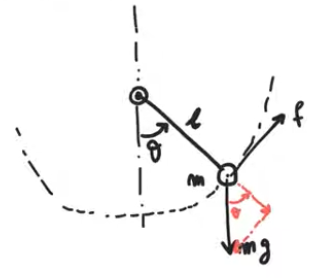
\includegraphics[width=\picwid]{pendolo.png}
 % pendolo.png: 316x278 px, 96dpi, 8.36x7.35 cm, bb=0 0 237 208
 \label{Fig.:pendolo_semplice}
\end{figure}

Si applica alla massa una forza $f$ tangente alla traiettoria della stessa, sul
pendolo agisce inoltre la forza peso $mg$ con $g$ l'accelerazione di gravità
nel punto in cui si trova il pendolo.

Il momento di inerzia $J$ di un pendolo di massa $m$ e lunghezza $l$ è pari a
$ml^2$.
Le coppie $\tau_n$ sono considerate positive se concordi all'asse uscente dal
piano di disegno (regola della mano destra).
La forza peso agisce sempre in direzione costante verso il basso, va scomposta
lungo due componentio e calcolare la coppia utilizzando la componente tangente
alla traiettoria dunque $lmg\sin\theta$.

$$
ml^2\ddot\theta = \sum_n{\tau_n} = lf - lmg\sin\theta
$$
